% Drawing 74/04-9 -- folder 74, batch 04, archive page 76 (PDF page 77).
% Transcription: un cube de revêtements, flèches marquées de leur degré (2 ou 3). Sommets lisibles : « $\tau$ = diagonales » relié par 2 à « sommets » ; « côtés » ; « rep.\ sym. » ; « sommets orientés $\simeq$ côtés $\simeq$ repères » ; $\varepsilon$ ; « triangles inscrits » ; « $\varepsilon' = \varepsilon \wedge \omega$, triangles coinscrits » ; « $\varepsilon \times \omega$, triangles inscrits orientés » ; « $\omega = \omega(\tau)$, orientations » ; le point $e$. Les flèches convergent vers $e$ ; plusieurs flèches et étiquettes du coin supérieur gauche sont surchargées et illisibles.
% Kind: cube of coverings (arrow diagram). Method 2 (schematic redraw from the facsimile). Status: partial.
% Notes: Labels placed where they stand (at \small, the figure drawn at 1.6 mm per unit), arrows as seen with their degrees 2 or 3; they converge on e. sommets -> tau = diagonales (2); tau = diagonales -> e (3); sommets orientés = côtés = repères -> sommets (2), -> côtés (2), -> rep. sym. (long arrow), and down to epsilon x omega; côtés -> epsilon; epsilon -> e (2); rep. sym. -> tau = diagonales (2); a vertical stroke from rep. sym. down to omega = omega(tau); a vertical arrow down to epsilon' = epsilon wedge omega; triangles inscrits -> e (2, bold); epsilon x omega -> epsilon' = epsilon wedge omega, triangles coinscrits (2, bold), -> triangles inscrits (2, doubled on the page); triangles inscrits orientés -> omega = omega(tau), orientations (2); omega -> e (2). Struck out and omitted: the scribbles over the upper left corner (around « tau = diagonales », a struck word and two struck arrows there). Still differs: which arrows carry which degree near the overwritten corner, and where the arrows start inside the cluster of labels at the top right, are readings. Redrawn 2026-11-09 (issue 128): to check again. Overlay check 2026-11-13 (issue 147, Claude claude-opus-5-5): the redraw, rasterised by the skill's previewer (not compiled: no TeX in the session), laid over the 300 dpi colour crop of the scan (261 ppi). The nodes and the arrows lie on their ink to within 1 to 3 units. Still differs, as said above: near the overwritten upper left corner which arrow carries which degree, and where the arrows start in the cluster of labels at the top right, are readings. It is an arrow diagram, which the editor prefers set as LaTeX (tikz-cd or array) in the transcription; as a redraw it stays partial.
% Coordinates: 1 unit = 1.6 mm = 1/100 of the crop width (bbox in page fractions: [0.33, 0.46, 0.75, 0.61]).
% Redrawn by Claude (claude-opus-5-5), issue #73, 2026-11-09; not checked by a human; not compiled (no TeX in the session).
% Checked by Claude (claude-opus-5-5) 2026-11-13 (issue #147): overlaid on the 300 dpi colour facsimile; not compiled (no TeX in the session). Status: partial.
% Rights: reproduces part of the work -- behind RENDER_TRANSCRIPTS, never published by itself.
\documentclass[tikz,border=3pt]{standalone}
\usepackage{amsmath,amssymb}
\usetikzlibrary{patterns,arrows.meta}
\tikzset{pencil/.style={black!45}, struck/.style={black!35}, mark/.style={circle,draw,inner sep=1.3pt}, pt/.style={circle,fill,inner sep=0.9pt}, opt/.style={circle,draw,fill=white,inner sep=1.1pt}}
\begin{document}
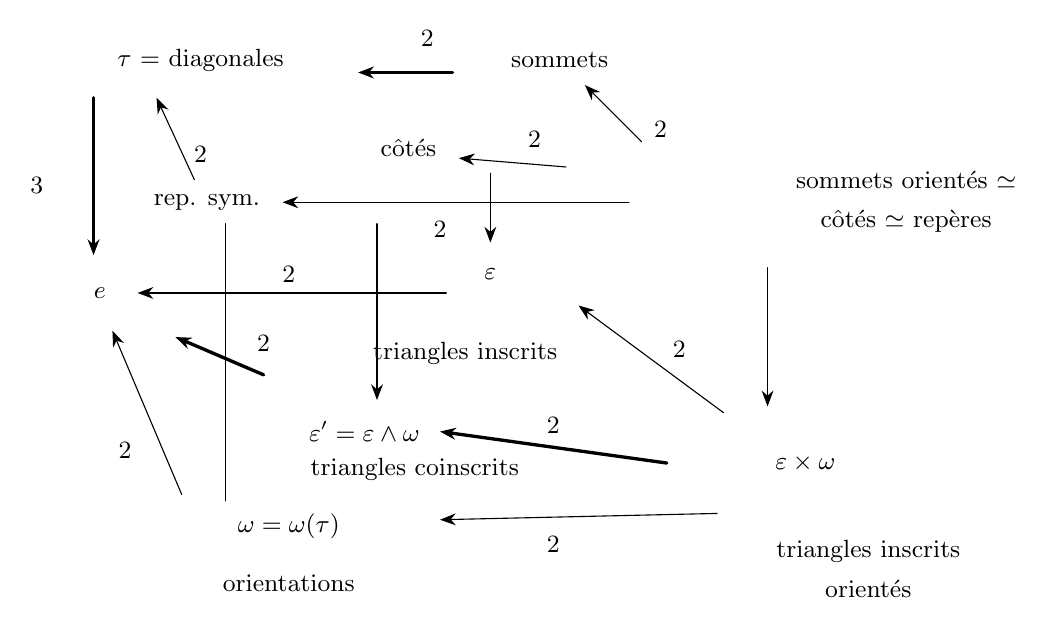
\begin{tikzpicture}[x=1.6mm,y=1.6mm,line cap=round,line join=round,font=\scriptsize]
\node[inner sep=1pt] at (19,-4) {\small $\tau$ = diagonales};
\node[inner sep=1pt] at (47.5,-4) {\small sommets};
\draw[-{Stealth[length=2mm]},very thick] (39,-5) -- (31.5,-5);
\node[inner sep=1pt] at (37,-2.3) {\small $2$};
\node[inner sep=1pt] at (35.5,-11) {\small côtés};
\draw[-{Stealth[length=2mm]}] (48,-12.5) -- (39.5,-11.8);
\node[inner sep=1pt] at (45.5,-10.3) {\small $2$};
\node[inner sep=1pt] at (19.5,-15.3) {\small rep. sym.};
\draw[-{Stealth[length=2mm]}] (53,-15.3) -- (25.5,-15.3);
\node[inner sep=1pt] at (75,-13.5) {\small sommets orientés $\simeq$};
\node[inner sep=1pt] at (75,-16.8) {\small côtés $\simeq$ repères};
\draw[-{Stealth[length=2mm]}] (54,-10.5) -- (49.5,-6);
\node[inner sep=1pt] at (55.5,-9.5) {\small $2$};
\node[inner sep=1pt] at (11,-22.5) {\small $e$};
\draw[-{Stealth[length=2mm]},very thick] (10.5,-7) -- (10.5,-19.5);
\node[inner sep=1pt] at (6,-14) {\small $3$};
\draw[-{Stealth[length=2mm]}] (18.5,-13.5) -- (15.5,-7);
\node[inner sep=1pt] at (19,-11.5) {\small $2$};
\node[inner sep=1pt] at (42,-21) {\small $\varepsilon$};
\draw[-{Stealth[length=2mm]}] (42,-13) -- (42,-18.5);
\node[inner sep=1pt] at (38,-17.5) {\small $2$};
\draw[-{Stealth[length=2mm]}] (38.5,-22.5) -- (14,-22.5);
\node[inner sep=1pt] at (26,-21) {\small $2$};
\draw (21,-17) -- (21,-39);
\draw[-{Stealth[length=2mm]}] (33,-17) -- (33,-31);
\node[inner sep=1pt] at (40,-27.3) {\small triangles inscrits};
\draw[-{Stealth[length=2mm]},very thick] (24,-29) -- (17,-26);
\node[inner sep=1pt] at (24,-26.5) {\small $2$};
\node[inner sep=1pt] at (32,-33.5) {\small $\varepsilon'=\varepsilon\wedge\omega$};
\node[inner sep=1pt] at (36,-36.5) {\small triangles coinscrits};
\node[inner sep=1pt] at (67,-36) {\small $\varepsilon\times\omega$};
\draw[-{Stealth[length=2mm]},very thick] (56,-36) -- (38,-33.5);
\node[inner sep=1pt] at (47,-33) {\small $2$};
\draw[-{Stealth[length=2mm]}] (60.5,-32) -- (49,-23.5);
\node[inner sep=1pt] at (57,-27) {\small $2$};
\draw[-{Stealth[length=2mm]}] (64,-20.5) -- (64,-31.5);
\node[inner sep=1pt] at (72,-43) {\small triangles inscrits};
\node[inner sep=1pt] at (72,-46) {\small orientés};
\draw[-{Stealth[length=2mm]}] (60,-40) -- (38,-40.5);
\node[inner sep=1pt] at (47,-42.5) {\small $2$};
\node[inner sep=1pt] at (26,-41) {\small $\omega=\omega(\tau)$};
\node[inner sep=1pt] at (26,-45.5) {\small orientations};
\draw[-{Stealth[length=2mm]}] (17.5,-38.5) -- (12,-25.5);
\node[inner sep=1pt] at (13,-35) {\small $2$};
\end{tikzpicture}
\end{document}
